\chapter{Introduction}
\label{chap:intro}

\section{Motivation \& Background}
\label{sec:motivation}

\subsection{The Machine Learning Context}
Machine Learning (ML) is a branch of Artificial Intelligence (AI) that studies algorithms and systems able to learn from data and improve their performance on tasks without being explicitly programmed for every detail. While traditional programming requires a human to specify every rule, ML uses data to infer models that map inputs to outputs or discover hidden patterns.

As the field has matured, a clear taxonomy of paradigms has emerged. As illustrated in Figure~\ref{fig:ml_taxonomy}, ML is generally categorized into three main branches:
\begin{enumerate}
  \item \textbf{Supervised Learning:} The algorithm learns from labeled data (input-output pairs) to predict future outcomes (e.g., Classification, Regression).
  \item \textbf{Reinforcement Learning:} An agent learns to make sequences of decisions by interacting with an environment to maximize a reward.
  \item \textbf{Unsupervised Learning:} The algorithm identifies patterns and structures in unlabeled data.
\end{enumerate}

\begin{figure}[H]
  \centering
  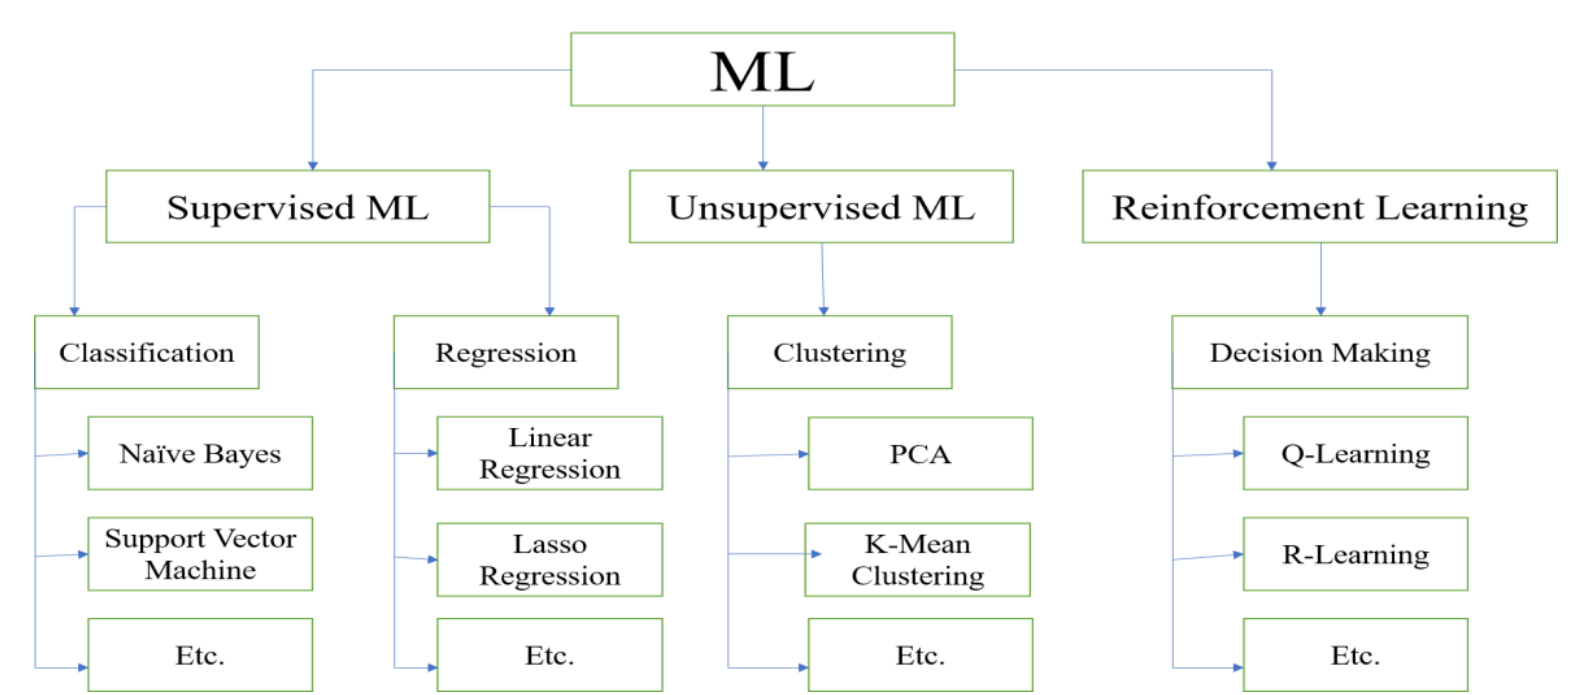
\includegraphics[width=0.85\linewidth]{images/ML_types.png}
  \caption{Taxonomy of common machine-learning paradigms and representative algorithms.}
  \label{fig:ml_taxonomy}
  \source{Compiled by the author}
\end{figure}

\subsection{The Role of Clustering in Unsupervised Learning}
This research focuses specifically on \textbf{Unsupervised Learning}, and more precisely, on Clustering. Unlike supervised methods, clustering algorithms do not have access to "ground truth" labels during training. Their objective is to discover inherent structures by grouping similar observations together based on geometric or statistical properties.

Clustering is fundamental for exploratory data analysis, customer segmentation, and anomaly detection. However, because these algorithms rely heavily on the geometric structure of the data (distances, densities, and distributions), they are highly sensitive to data quality and distribution. Common algorithms include:
\begin{itemize}
  \item \textbf{K-Means:} Partitioning data into $k$ groups by minimizing variance within clusters.
  \item \textbf{Hierarchical Clustering:} Building a tree of clusters (dendrogram) based on distance connectivity.
\end{itemize}

\subsection{The Data Dilemma: Privacy vs. Utility}
While algorithms like K-Means and Hierarchical Clustering are powerful, their development is increasingly hindered by a critical bottleneck: access to high-quality data.

In sectors such as healthcare, finance, and government, data contains sensitive personal information (PII). Regulations such as the General Data Protection Regulation (GDPR) in Europe strictly limit how this data can be shared and used. This creates a "Privacy vs. Utility" trade-off:
\begin{itemize}
  \item \textbf{High Privacy:} Data is locked away, stifling research and model development.
  \item \textbf{High Utility:} Data is shared freely, risking privacy breaches and legal non-compliance.
\end{itemize}

\subsection{Synthetic Data as a Solution}
To resolve this conflict, the concept of Synthetic Data has emerged as a leading solution. Synthetic data is artificially generated information that replicates the statistical properties, structure, and correlations of a real dataset without containing any information about real individuals.

Ideally, synthetic data offers the best of both worlds: 1. Privacy: It is impossible to re-identify individuals because the records are fictitious. 2. Utility: Statistical analyses (like clustering) performed on the synthetic data should yield the same conclusions as if they were performed on the real data \cite{nowok2016, qian2024}.

However, a critical question remains: \textit{Does the generation process distort the complex geometric structures required for clustering?} If a synthetic data generator (such as the CART method) alters the distances or densities between points, clustering algorithms may fail to detect the correct groups, rendering the synthetic data useless for this specific task.

\section{Purpose}
\label{sec:purpose}
The primary purpose of this research is to evaluate the utility of synthetic data for clustering tasks. Specifically, this project extends the work of Chen Xinnuo \cite{chen2025} to systematically compare how well K-Means and Hierarchical Clustering perform on synthetic data generated via the Classification and Regression Trees (CART) method (implemented in the \texttt{synthpop} R package).

We aim to answer three specific research questions:
\begin{enumerate}
  \item \textbf{Detection Capability:} Can clustering algorithms correctly identify the optimal number of clusters ($k$) in synthetic data as well as they do in real data?
  \item \textbf{Algorithm Robustness:} Which algorithm is more resilient to the distortions introduced by the synthetic generation process? We hypothesise that Hierarchical Clustering may be more robust than K-Means in non-normal distributions.
  \item \textbf{Quantification of Degradation:} To what extent does the CART generation method degrade the geometric properties (separability, density) of the clusters?
\end{enumerate}

To answer these questions, we have developed a reproducible pipeline that generates 1,800+ datasets varying in sample size ($N$), cluster separation, noise levels, and probability distributions (Normal vs. Gamma), allowing for a rigorous statistical comparison.

\section{Structure of the document}
\label{sec:structure}
The remainder of this report is organized as follows:
\begin{itemize}
  \item \textbf{Chapter 2: Methods} details the mathematical formulations of K-Means and Hierarchical Clustering and describes the synthetic data generation via CART. It also defines the novel structural fidelity metrics and the simulation pipeline used to evaluate algorithm robustness.
  \item \textbf{Chapter 3: Results} presents the empirical analysis, including PCA and t-SNE visualizations alongside cluster detection success rates. It further quantifies geometric degradation using the Gini coefficient, Mean Centroid Distance, and Mean Variance Difference metrics.
  \item \textbf{Chapter 4: Conclusions} synthesizes the findings, highlighting the superior robustness of Hierarchical Clustering for skewed synthetic data. It discusses the practical implications for the privacy-utility trade-off, acknowledges limitations, and proposes future research directions.
\end{itemize}